\chapter{Braid groups}
\label{chapter2}
 
\section{The Artin braid group}

Ambient isotopy gives an equivalence relation for $n$-braids. The Artin braid group $B_n$ is the group whose elements are equivalence classes of $n$-braids under the equivalence of ambient isotopy and whose group operation is composition of braids.

Let $X$ be a space and $X^n$ be its product space with product topology. Define 
\begin{equation}
\label{eq:7}
  \text{Conf}_n(X) = \{ (x_1, \ldots, x_n) \ |\ (x_i \ne x_j) \text{ for all } i \ne j\}.
\end{equation}
This subspace $\text{Conf}_n(X)$ of $X^n$ is called the ordered $n$th configuration space of $X$. An alternative formulation gives $\text{Conf}_n(X) = \{ f \ | \ \mathbf{n} \to X \text{ is injective} \}$, where $\mathbf{n} = \{1, \ldots, n\}$. In other words, $\text{Conf}_n(X)$ is the subspace made of ordered $n$-tuples of distinct points in $X$.

Let $S_n$ be the symmetric group. The unordered $n$th configuration space $\text{UConf}_n(X)$ is defined as the quotient $\text{Conf}_n(X)/S_n$. That is, points in $\text{UConf}_n(X)$ are equivalence classes of points in $\text{Conf}_n(X)$ under the equivalence relation of permutation.

\begin{theorem}
\label{sec:artin-braid-group-1}
The fundamental group of $\text{UConf}_n(\R^2)$ is the braid group $B_n$. 
\begin{equation}
\label{eq:9}
B_n \cong \pi_1(\text{UConf}_n(\R^2)).
\end{equation}
\end{theorem}

As usual, let $I$ be the unit interval. A path $p: I \to \text{UConf}_n(\R^2)$ describes trajectories of $n$ particles in $\R^2$ except each particle moves in its own copy of $\R^2$. The condition of distinctness of points in the definition of $\text{UConf}_n(\R^2)$ makes sure no two particles meet (or rather, have the same coordinates in $\R^2$).

Let $p(0) = \{ (0,1), \ldots, (0,n) \}$ be the initial position of the particles (or one end of each strand of the braid). One may let $p(0)$ be the basepoint (the choice does not matter since $\text{UConf}_n(\R^2)$ is connected). Let $p(1) = \{ (1,1), \dots, (1,n) \}$ be the final positions of the particles.

The homotopy of these paths corresponds to isotopy of braids. Each trajectory describes a strand in the braid. One may connect the corresponding ends of strands in pairs and form loops. Under the homotopy of loops, we have $B_n = \pi_1(\text{UConf}_n(\R^2))$.

\begin{remark}
\label{sec:artin-braid-group-3}
The choice of the final position $p(1)$ is only to facilitate our mental picture of a braid. One may define $p(1)$ to be any other point on $\text{UConf}_n(\R^2)$.
\end{remark}

\begin{remark}
The above arguments are incomplete and non-rigorous. However, they should give an idea of the proof.
\end{remark}

One may look at $B_n$ purely algebraically guided by our mental picture of a braid. Consider the $n$-braids $\sigma_1,\ldots, \sigma_{n-1}$, where $\sigma_i$ is the $n$-braid in which the $i$th strand crosses over the $(i+1)$the strand while every other strand runs parallel (that is, there is no other double point or crossing). Impose the following relations:

\begin{align}
\label{eq:4}
  \sigma_i\sigma_j &= \sigma_j\sigma_i \hspace*{3.6em}\text{for } i-j \geq 2, \\
  \sigma_i\sigma_{i+1}\sigma_i &= \sigma_{i+1}\sigma_i\sigma_{i+1} \hspace*{1em}\text{for } 1 \leq i \leq n-2.
\end{align}

Let $R$ be the set of the above relations. Let $S = \{\sigma_1,\ldots, \sigma_{n-1}\}$. 

\begin{theorem}
\label{sec:artin-braid-group-4}
The group $\langle S : R \rangle$ is the braid group $B_n$.
\end{theorem}

Observe that the set of relations, $R$, give braid isotopies (ambient isotopy in $\R^3$ and planar isotopy in $\R^2$) and are called the braid relations.


\begin{theorem}
\label{sec:artin-braid-group-6}
Let $G$ be a group. Suppose $s_1, \ldots, s_{n-1} \in G$ satisfy the braid relations $R$. Then there is a unique homomorphism $\psi : B_n \to G$ such that $\psi(\sigma_i) = s_i$ for all $1 \leq i \leq n-1$. 
\end{theorem}

\begin{proof}
\label{sec:artin-braid-group-7}
Let $F_n$ be the free group generated by $\sigma_1,\ldots, \sigma_{n-1}$. By the universal property of free groups, there is a unique homomorphism $\psi^{\prime}: F_n \to G$ such that $\psi^{\prime}(\sigma_i) = s_i$ for all $1 \leq i \leq n-1$. This homomorphism induces the homomorphism $\psi : B_n \to G$ provided the braid relations $R$ are preserved. One easily checks that $\psi(r) = \psi(r^{\prime})$ for each braid relation $r = r^{\prime}$.
\end{proof}

The converse to the above theorem is obvious. Given a homomorphism $\psi : B_n \to G$ such that $\psi(\sigma_i) = s_i$, one checks that $\{s_1, \ldots, s_{n-1}\}$ satisfy the braid relations $R$.

Let $\beta_n \in B_n$ be a braid (a more accurate description would be: $\beta_n$ is an equivalent class of $n$-strand braids under isotopy). The closed braid $\overline{\beta_n}$ is the link obtained by connecting the corresponding ends in pairs.

Let us give an orientation to a braid $\beta \in B_n$: all strands are considered being directed from top to bottom. Then the closed braid $\overline{\beta_n}$ is an oriented link. Henceforth, we adopt this orientation as a convention.

\begin{theorem}[Alexander]
\label{sec:artin-braid-group}
Any oriented link diagram in $\R^2$ is isotopic to a closed braid.
\end{theorem}

The original proof given by Alexander is straightforward but has some drawbacks. Nevertheless, we sketch the essence of the proof below. Recall that a polygonal link is a geometric link whose components are closed broken lines.

The idea of the proof goes this way: Any link in $\R^3$ is ambient isotopic to a polygonal link. Therefore, it suffices to prove that any oriented polygonal link $L$ is ambient isotopic to a closed braid. Let $D$ be a polygonal oriented link diagram. We choose a point $P$ on the plane not lying on the $D$. This gives an axis $l$ passing through $P$ perpendicular to the plane. Then we begin at any point on $D$ and move counterclockwise around the axis $l$. The plan is to have the link wind around the axis in one direction (that is, counterclockwise). If the link begins to wind around the axis incorrectly we throw the strand over the axis so that it keeps winding in the right direction. Suppose $AC$ is the edge in $D$ that is winding around $l$ in the incorrect direction. Then we replace $AC$ with two new edges $AA^{\prime}$ and $A^{\prime}C$. We keep doing this for any edge in $D$ that winds incorrectly. Since there are finitely many edges in $L$, this process stops with all edges winding counterclockwise. Then we draw a radial line from $P$ intersecting the edges transversely at finitely many points. From this we get a braid; the points of intersection give the endpoints of the braid.

Despite the simplicity and the straightforwardness of the proof, it is difficult and impractical to write a computer program based upon it. We shall see a different proof originally due to Yamada but improved later by Vogel. This proof has two major advantages: (1) We can write an efficient computer program for putting knots or links in closed braid form; (2) It has a beautiful corollary that reveals structure about link diagrams.

We will use the book of Kassel-Turaev \cite{kassel2008braid} as our reference.

\begin{definition}
\label{sec:artin-braid-group-8}
Smoothing all crossings of a given oriented link diagram $D$ in the standard orientation-preserving way yields a union of disjoint oriented loops (topological circles). These circles are called Seifert circles of the diagram $D$.
\end{definition}

The following diagram is how we smooth the crossings.

\begin{figure}[h]
  \centering
  \includegraphics[scale=.35]{images/smoothing.png}
\end{figure}

\begin{definition}
\label{sec:artin-braid-group-9}
Any two disjoint oriented circles on the sphere $S^2$ bound an annulus in $S^2$. These circles are said to be incompatible if their orientation is induced by an orientation of this annulus. Otherwise, these circles are compatible.
\end{definition}

\begin{remark}
Two oriented concentric cirles in $\R^2$ are compatible if they both are oriented clockwise or both counterclockwise, and if they are not concentric in $\R^2$, they are only compatible when they have opposite orientations otherwise incompatible.
\end{remark}

\begin{figure}[h]
  \centering
  \includegraphics[scale=.35]{images/incompatibility.png}
\end{figure}

In the above, circles $C_1$ and $C_2$ are compatible to each other but incompatible to $C_3$.

Let $n_S(D)$ denote the number of Seifert circles of an oriented link diagram $D$. The compatibility of Seifert circles is defined in the same way (above). Let $n_{i}(D)$ denote the number of pairs of incompatible Seifert circles of $D$.

In the diagram $D$, forget the information of over/undercrossing. In other words, each crossing becomes a vertex of degree $4$. Denote this 4-valent digraph by $D_G$. The edges and faces of $D_G$ are defined the obvious way by considering $D_G$ as a planar graph.

\begin{remark}
\label{sec:artin-braid-group-11}
In general, $D_G$ may be disconnected and have self-loops. Thus, edges of $D_G$ are either arcs or circles in $\R^2$.
\end{remark}

\begin{definition}
\label{sec:artin-braid-group-12}
A face $f$ of $D_G$ is said to be adjacent to an edge $e$ of $D_G$ if $e$ forms a part of the boundary of the closure of $f$. A face $f$ is said to be adjacent to a Seifert circle $S$ of $D$ if $f$ is adjacent to at least one edge of $D$ contained in $S$.
\end{definition}

\begin{definition}
\label{sec:artin-braid-group-13}
A face $f$ of $D_G$ is said to be defect if there exist distinct edges $e_1, e_2$ of $D_G$ such that $f$ is adjacent to both $e_1, e_2$, and the Seifert circles $S_1, S_2$ of $D$ going along $e_1, e_2$ are distinct and incompatible.
\end{definition}

\begin{definition}
\label{sec:artin-braid-group-14}
A reduction arc $c \subset \R^2$ in a face $f$ of $D_G$ is an oriented arc leading from a point on edge $e_1$ to a point on edge $e_2$ and lying (except the endpoints, of course) in a face $f$ of $D_G$.
\end{definition}

\begin{definition}
\label{sec:artin-braid-group-15}
Let $a_1, a_2$ be two arcs belonging to two distinct incompatible Seifert circles $S_1, S_2$. Suppose there is a reduction arc $c$ from a point on $a_1$ to a point on $a_2$. Then a Yamada-Vogel reducing move, denoted by $\mathcal{Y}$ (or $\mathcal{Y}^+$), is the pulling of the arc $a_1$ over the arc $a_2$ along $c$ creating two new double points (crossings).
\end{definition}

\begin{remark}
\label{sec:artin-braid-group-16}
Check that $\mathcal{Y}^+$ is a variant of $\mathcal{R}^2$. Let $-c$ be the same arc $c$ with opposite orientation. Performing $\mathcal{Y}^+$ along $-c$ yields a similar diagram except the arc $a_2$ is now above $a_1$ at the crossings. The inverse of the move $\mathcal{Y}^+$ is denoted by $\mathcal{Y}^-$.  Obviously $\mathcal{Y}^{\pm 1}$ does not change the isotopy class of an oriented link diagram.
\end{remark}

Let $D^{\prime}$ be the diagram obtained from a oriented link diagram $D$ by a single reducing move $\mathcal{Y}^+$. Denote this process by $D \xrightarrow{\mathcal{Y}^+} D^{\prime}$. 

\begin{lemma}
\label{l1}
Let $D$ and $D^{\prime}$ be two oriented link diagrams in $S^2$ such that $D \xrightarrow{\mathcal{Y}^+} D^{\prime}$. Then $n_S(D^{\prime}) = n_S(D)$ and $n_{i}(D^{\prime}) = n_{i}(D) - 1$.
\end{lemma}

\begin{proof}
  Suppose $S_1, S_2$ are two distinct and incompatible Seifert circles of $D$ involved in the reducing move $\mathcal{Y}^{+}$. We may draw two non-concentric circles $S_1, S_2$ with the same orientation (say, counterclockwise). Recall that a reducing move $\mathcal{Y}^+$ is performed by pulling an arc $a_1$ of $S_1$ over another arc $a_2$ of $S_2$ along a reducing arc $c$. By making use of planar isotopy, we can make sure that no other Seifert circles of $D$ is affected by this move. Indeed, there is a planar region between arcs $a_1$ and $a_2$ where $\mathcal{Y}^+$ is performed and in which no Seifert circles of $D$ pass through. Suppose the reducing move $\mathcal{Y}^{+}$ gives rise to two new Seifert circles $S_0$ and $S_{\infty}$ of $D^{\prime}$. Observe that all other Seifert circles of $D$ are left untouched. Thus, the first part of the lemma follows.
  
Let $D_1, D_2$ be the disjoint disks bounded by the Seifert circles $S_1, S_2$. Let $d_i$ denote the number of Seifert circles of $D$ lying in the open disk $D_i^{\circ} = D_i - \partial D_i$. Let $d$ be the number of Seifert circles of $D$ lying in the annulus $S^2 - (D_1 \cup D_2)$ and incompatible with $S_1$. Let $k$ be the number of pairs of incompatible Seifert circles of $D$ both distinct from $S_1, S_2$.

\begin{claim}
  The number of pairs of incompatible Seifert circles of $D$ is given by $n_{i}(D) = k + d_1 + d_2 + 2d + 1$.
\end{claim}

It suffices to show that the number of pairs of incompatible Seifert circles of $D$ including $S_1$ or $S_2$ or both is equal to $d_1 + d_2 + 2d + 1$. Observe that, for $i = 1, 2$, an oriented circle in $D_i^{\circ}$ can only be incompatible with either $S_1$ or $S_2$, but not with both. This gives the contribution $d_1 + d_2$. Next, observe that an oriented circle in $S^2 - (D_1 \cup D_2)$ is incompatible with $S_1$ if and only if it is incompatible with $S_2$. This contributes $2d$. Since $S_1$ and $S_2$ are incompatible, we add one.

\begin{claim}
  The number of pairs of incompatible Seifert circles of $D$ is given by $n_i(D^{\prime}) = k + d_1 + d_2 + 2d$.
\end{claim}

A similar argument works for this one. Hence $n_i(D^{\prime}) = n_i(D) - 1$.
\end{proof}

\begin{remark}
\label{sec:artin-braid-group-17}
  In the proof above, we drew two non-concentric circles $S_1, S_2$. One may also check for concentric circles but is not really necessary.
\end{remark}

Cutting $S^2$ along the Seifert circles of $D$ disintegrates $S^2$ into a union of surfaces. Each of these surfaces are taken to have a boundary (which is a Seifert circle of $D$). Let $\Omega$ denote the union of these surfaces. See that $\Omega$ is a compact surface with boundary.

For each crossing $x$ of $D$, let $\gamma_{x}$ denote a line segment near $x$ joining the two Seifert circles involved in the crossing $x$. Observe that any two $\gamma_x$ and $\gamma_y$ are disjoint and each $\gamma_x$ lie in a connected component of $\Omega$.

\begin{lemma}
\label{sec:artin-braid-group-18}
Let $n_i(D) > 0$. There exist a connected component $F$ of $\Omega$ and two Seifert circles in $\partial F$ whose orientation is induced by an orientation on $F$.
\end{lemma}

\begin{proof}
  Since $n_i(D) > 0$, there is at least a pair of two incompatible Seifert circles of $D$. Let $S_1, S_2$ be two such circles and $c \subset \R^2$ be an oriented arc from a point on $S_1$ to a point on $S_2$. Assume that $c$ meets each Seifert circle of $D$ transversely in at most one point. If $c$ meets a Seifert circle in more than one point, we can adjust using planar isotopy so that $c$ meets it in only one point. See that the point of meetings of $c$ with these circles form a finite subset of $c$ including the endpoints. As we move along $c$, see that at each crossing the corresponding Seifert circle is directed either to the left or to the right of $c$. Since $S_1, S_2$ are incompatible to begin with, their directions at the endpoints of $c$ must be opposite. We deduce that among the crossings of $c$ with the Seifert circles, there are two that lie consecutively and at which the directions of the corresponding Seifert circles are opposite. It follows that the connected component $F$ of $\Omega$ containing the subarc of $c$ between two such crossings satisfies the condition given in the lemma.
\end{proof}

\begin{lemma}
  \label{l2}
An oriented link diagram $D$ in $\mathbb{R}^2$ has a defect face if and only if $n_i(D) \ne 0$.
\end{lemma}

\begin{proof}
  The forward direction of the lemma is obvious from the definition of a defect face. Therefore, we only prove that if $n_i(D) > 0$, then $D$ has a defect face. By the previous lemma, we can consider a connected component $F$ of $\Omega$ such that there are at least two Seifert circles in $\partial F$ whose orientation is induced by an orientation on $F$. We fix such an orientation on $F$. We call a Seifert circle in $\partial F$ positive if its orientation is induced by the one on $F$ and negative otherwise.

  By assumption, there are at least two positive Seifert circles in $\partial F$. If $F$ contains no segments $\gamma_x$, then the interior $F^{\circ} = F - \partial F$ is a face of $D_G$ adjacent to at least two positive Seifert circles in $\partial F$. Hence this face is a defect face. Suppose $F$ contains certain segments $\gamma_x$. We remove all such segments from $F$ and obtain a subsurface $F^{\prime}\subset F$. See that any connected component $f$ of $F^{\prime}$ is adjacent to at least one segment $\gamma_x$ and the interior of $f$ is a face of $D_G$. See that each $\gamma_x \subset F$ connects a positive Seifert circle in $\partial F$ with a negative one. Thus $f$ is adjacent to at least one positive and at least one negative Seifert circle.

  If $f$ is adjacent to at least two positive or to at least two negative Seifert circles, then $f$ is a defect face. Suppose each connected component $f$ of $F^{\prime}$ is adjacent to exactly one positive and exactly one negative Seifert circle. Observe that if we move from $f$ to a neighboring component of $F^{\prime}$ across some $\gamma_x\subset F$, we only meet the same Seifert circles. Since $F$ is connected, we can move in this way from any component of $F^{\prime}$ to any other component. Thus $\partial F$ contains exactly one positive and one negative Seifert circle, which contradicts our assumptions. It follows that $D$ has a defect face.
\end{proof}

\begin{lemma}
  \label{l3}
  Let $D$ be a oriented link diagram with $n_i(D) = 0$. Then $D$ is isotopic in the sphere $S^2$ to a closed braid diagram.
\end{lemma}

\begin{proof}
  If a connected component of $\Omega$ more than two boundary components, then two of them must be incompatible in $S^2$ so that $n_i(D) \ne 0$. Since $n_i(D) = 0$, we conclude that each connected component of $\Omega$ has at most two components. Observe that a compact and connected subsurface of $S^2$ whose boundary has at most two components must be either a disk or an annulus. Thus $\Omega$ contains only disks and annuli.

  Next the Seifert circles of $D$ can be transformed (using isotopy in $S^2$) into a union of disjoint concentric circles in $\R^2$. Using this isotopy in $S^2$, one may assume from the beginning that the Seifert circles of $D$ are concentric circles in $\R^2$. Since $n_i(D)= 0$, these Seifert circles are oriented either all clockwise or all counterclockwise.

  We assume all the Seifert circles are oriented counterclockwise. If they are oriented clockwise, we may push all of them across infinity to obtain counterclockwise orientation. By planar isotopy, we assume that the segments $\gamma_x$ are all radial. The resulting diagram is then a closed braid diagram and we are done.
\end{proof}

\begin{proof}[Proof of Theorem \ref{sec:artin-braid-group}]
\label{sec:artin-braid-group-19}
  Let $D$ be an oriented link diagram. If $n_i(D) = 0$, we are done. If $n_i(D) > 0$, there is a defect face. Then we perform a $\mathcal{Y}^+$ on $D$ to obtain $D^{\prime}$ and we have $n_i(D^{\prime}) = n_i(D) - 1$. Indeed, we have a sequence of isotopic oriented link diagrams connected by $\mathcal{Y}^+$ moves: 
\begin{equation}
\label{eq:11}
D \xrightarrow{\mathcal{Y}^+} D^{\prime} \xrightarrow{\mathcal{Y}^+} \cdots \xrightarrow{\mathcal{Y}^+} D_0,
\end{equation}
where $n_i(D_0) = 0$. Then $D_0$ is a closed braid diagram.
\end{proof}

\begin{remark}
\label{sec:artin-braid-group-20}
Observe that the length of any sequence of reducing moves $\mathcal{Y}^+$ required to transform $D$ to a closed braid is given by $n_i(D)$.
\end{remark}

\begin{definition}
  The braid index of a link $L$ is the minimum number $n$ such that there exists a braid $\beta \in B_n$ whose closure $\overline{\beta}$ represents $L$.
\end{definition}

\begin{corollary}
  The minimum number of Seifert circles in any diagram of a link $K$ is equal to the braid index of $K$.
\end{corollary}

This follows from Lemma \ref{l1}.

Notwithstanding that Alexander's theorem guarantees that any oriented link can be realized as a closed braid, it has no say on the uniqueness of the closed braid and as such, it has little use in studying knots from braid groups. Markov's theorem states that any two closed braids expressing the same link are mutually related by successive applications some special moves, which we describe below.

Let $\beta \in B_n$ be a braid. A Markov move is defined to be any one of the following types
\begin{enumerate}
\item\label{item:6} Conjugation: the transformation $\beta \to \alpha \beta \alpha^{-1}$ or inverse, for any $\alpha \in B_n$
\item\label{item:10} The move $\beta \to \beta \sigma_n^{\pm 1}$ where $\beta \in B_n$ and $\beta \sigma_n^{\pm 1} \in B_{n+1}$,
\item\label{item:12} Isotopy in the braid group $B_n$ (given by the braid relations).
\end{enumerate}
\begin{theorem}[Markov]
    Two braids have isotopic closures in $\mathbb{R}^3$ if and only if these braids are related by a sequence of Markov moves.
  \end{theorem}
  The theorem can also be formulated in the following way:
\begin{theorem}[Markov]
\label{sec:markovs-theorem}
  Let $\beta$, $\beta^{\prime}$ be two closed braids representing the same oriented link $L$ in $\R^3$. Then there exists a sequence of closed braids, each of them representing $L$,
\begin{displaymath}
\beta = \beta_1 \to \beta_2 \to \cdots \to \beta_r = \beta^{\prime}
\end{displaymath}
such that each $\beta_{i+1}$ is obtained from $\beta_i$ by a single Markov move.
\end{theorem}

A proof of this theorem can be found here \cite{traczyk1998new}.

We say that two closed braids are Markov-equivalent or M-equivalent if they are related by a sequence of Markov moves. 

Markov's theorem gives us a tool to construct invariants for knots and links. Here we define Markov functions and show how link invariants can be constructed.

  \begin{definition}
  A Markov function with values in a set $E$ is a sequence of set-theoretic maps $\{ f_n: B_n \to E \}_{n\geq 1}$, satisfying the following conditions: 
\begin{enumerate}
\item\label{item:13} for all $n \geq 1$ and all $\alpha, \beta \in B_n$, 
\begin{displaymath}
f_n(\alpha \beta ) = f_n (\beta \alpha);
\end{displaymath} 
\item\label{item:14} for all $n \geq 1$ and all $\beta \in B_n$, 
\begin{displaymath}
f_n(\beta) = f_{n+1}(\sigma_n \beta) \text{ and } f_n(\beta) = f_{n+1}(\sigma_n^{-1} \beta).
\end{displaymath}
\end{enumerate}
\end{definition}

\begin{theorem}
  \label{markovisotopy}
  Any Markov function $\{ f_n : B_n \to E \}_{n \geq 1}$ determines an $E$-valued isotopy invariant $\hat{f}$ of oriented links in $\mathbb{R}^3$.
\end{theorem}
\begin{proof}
  Let $K$ be an oriented link in $\mathbb{R}^3$. Pick a braid $\beta \in B_n$ whose closure is isotopic to $K$ and set $\hat{f}(K) = f_n(\beta) \in E$. Check that $\hat{f}(K)$ does not depend on the choice of $\beta$. Indeed, if $\beta^{\prime} \in B_{n^{\prime}}$ is another braid whose closure is ambient isotopic to $K$, then $\beta$ and $\beta^{\prime}$ are M-equivalent (by Markov's theorem). It can be seen from M-equivalence and the definition of the Markov function that $f_n(\beta) = f_{n^{\prime}}(\beta^{\prime})$. The function $\hat{f}$ is an isotopy invariant of oriented links: if $K, K^{\prime}$ are isotopic oriented links in $\mathbb{R}^3$ and $\beta \in B_n$ is a braid whose closure is isotopic to $K$, then the closure of $\beta$ is also isotopic to $K^{\prime}$ and $\hat{f}(K) = f_n(\beta) = \hat{f}(K^{\prime})$.
\end{proof}

\section{The Burau representation}

Let $X$ be an object in a category $\A$. An automorphism of $X$ is an isomorphism from $X$ to itself. Automorphisms of $X$ form a group, called the automorphism group of $X$ and denoted by $\text{Aut}(X)$, whose operation is the composition of these isomorphisms.

\begin{propdef}
\label{sec:representations}
Let $X$ be a finite-dimensional vector space. The general linear group of $X$, denoted by $\text{GL}(X)$, is the automorphism group $\text{Aut}(X)$.
\end{propdef}

Suppose $X$ is an $n$-dimensional $\R$-vector space with a fixed basis. Then an automorphism of $X$ is an invertible linear transformation $X \to X$ which is defined by an invertible matrix of order $n\times n$. Then $\text{Aut}(X)$ is the group of all invertible matrices of order $n\times n$ with entries in $\R$, which is the usual general linear group denoted by $\text{GL}_n(\R)$.

In representation theory, we represent groups as automorphisms of a vector space $X$. Since an element of $\text{Aut}(X)$ is an invertible matrix, we are essentially representing a group as a set of invertible matrices, that is, mapping each element of a group to an invertible matrix. One sees that this map should then be a homomorphism. Such representations often reduces difficult group-theoretic problems to matrix manipulations, which are easier.

\begin{propdef}
  \label{sec:representations-1}
  A representation of a group $G$ on a vector space $X$ over a field $K$ is a homomorphism from $G$ to the automorphism group $\text{Aut}(X)$ of a vector space $X$, which is the general linear group $\text{GL}(X)$. The vector space $V$ is called the representation space of $G$ and the dimension of $V$ is called the dimension or degree of the representation.
\end{propdef}

More generally, one may define a group representation as a homomorphism from that group to any other group.

\begin{remark}
\label{sec:representations-2}
  In the discussion above, we have identified $\text{GL}(X)$ with $\text{GL}_n(\R)$. When $X$ is an $n$-dimensional vector space with underlying field $K$ with a chosen basis, we usually identify $\text{GL}(X)$ with $\text{GL}_n(K)$.
\end{remark}

Before going further, we state group representation in category-theoretic terms. Any group $G$ can be seen as a category $\mathcal{G}$ with one object which is the group itself. The elements of $G$ are seen as the morphisms in $\mathcal{G}$. Let $\A$ be an arbitrary category. A representation of $G$ in $\A$ is a functor from $\mathcal{G}$ to $\A$ taking $G$ to some object $X$ of $\A$. Then the functor takes the group elements of $G$ to automorphisms of $X$ establishing a homomorphism $G \to \text{Aut}(X)$. In our case, $\A$ is \textbf{FVect$_k$}, the category of finite dimensional vector spaces over a field $k$. 

\begin{definition}
\label{sec:representations-3}
  A group representation $\rho : G \to \text{GL}(X)$ is said to be faithful if $\rho$ is injective or equivalently, the kernel $\ker{\rho}$ is trivial.
\end{definition}

\begin{definition}
\label{sec:representations-4}
Let $\rho : G \to \text{GL}(X)$ be a group representation. A subspace $Y \subset X$ is said to be $G$-invariant if $\rho(g)y \in Y$ for all $g \in G, y \in Y$. The restriction of $\rho$ to $Y$ is called a subrepresentation. The trivial subspace $\{0\}$ and $X$ are trivial subrepresentations. The representation $\rho$ is said to be irreducible if all its subrepresentations are trivial; otherwise it is reducible.
\end{definition}

Equipped with this, we are ready to discuss the Burau representation of braid groups. We shall use Theorem \ref{sec:artin-braid-group-6} to great effect. If $s_1,\ldots, s_{n-1}$ are elements of a group $G$ satisfying the braid relations, then we have a braid representation $\rho : B_n \to G$ such that $\rho(\sigma_i) = s_i$.

First, we describe the Burau representation using explicit matrices. Let $\Uplambda = \mathbb{Z}[t, t^{-1}]$ be the ring of Laurent polynomials. Fix $n\geq 2$. For $i=1,2,\ldots, n-1$, set 
\begin{equation}
  U_i = \begin{pmatrix} I_{i-1} & 0 & 0 & 0 \\
    0 & 1-t & t & 0 \\
    0 & 1 & 0 & 0 \\
  0 & 0 & 0 & I_{n-i-1}\end{pmatrix},
\end{equation}
where $I_{i-1}$ is the identity (unit) matrix of order $i-1$ and so on. Observe that each $U_i$ have three blocks $I_{i-1}$, $U$ and $I_{n-i-1}$, where we have set 
\begin{equation}
\label{eq:8}
U = \begin{pmatrix} 1-t & t \\ 1 & 0 \end{pmatrix}.
\end{equation}

By the Cayley-Hamilton theorem, the $2 \times 2$ matrix $U$ over the ring $\Uplambda$ satisfies $U^2 - \text{tr}(U)U + \det(U)I_2 = 0$. Observe that the identity matrices also satisfy this equation. Exploiting the block form the matrix $U_i$, we deduce that $U_i^2 = \text{tr}(U_i)U_i + \det(U_i)I_n = 0$ for all $i$. Rewriting this equation as $U_i(U_i - (1-t)I_n) = tI_n$, see that $U_i$ is invertible over $\Uplambda$. From here, one finds the inverse of $U_i$.

\begin{proposition}
\label{sec:burau-representation-2}
The matrices $U_1, \ldots, U_{n-1}$ satisfy the braid relations:
\begin{align}
\label{eq:10}
  U_iU_j &= U_jU_i \hspace*{3.8em}\text{for } i-j \geq 2, \\
  U_iU_{i+1}U_i &= U_{i+1}U_iU_{i+1} \hspace*{1em}\text{for } 1 \leq i \leq n-2.
\end{align}
\end{proposition}

Exploiting the block form of $U_i$, one easily proves the proposition above. Since the $U_i$ satisfy the braid relations, we have a group homomorphism $\psi_n: B_n \to \text{GL}_n(\Uplambda)$ satisfying $\psi_n(\sigma_i) = U_i$. This is the Burau representation of the braid group $B_n$.

\begin{remark}
\label{sec:burau-representation-5}
  In the above, we wrote $GL_n(\Uplambda)$ to mean the group of invertible matrices of order $n\times n$ over ring $\Uplambda$. See that $\Uplambda$ is a commutative ring. Recall that by the definition of group representation, we are looking at homorphism $B_n \to GL(X)$ except in this case $X$ is a $\Uplambda$-module of rank $n$. The automorphisms of a $\Uplambda$-module are given by invertible matrices over $\Uplambda$. Thus, it makes sense to identify $\text{GL}(X)$ with $\text{GL}_n(\Uplambda)$.
\end{remark}

\begin{remark}
\label{sec:burau-representation-6}
Observe that $\det(U_i) = -t$ for all $i$. This implies that for any $\beta \in B_n$, we have $\det \psi_n(\beta) = (-t)^{\langle \beta \rangle}$, where $\langle \beta \rangle \in \Z$ is the image of $\beta$ under the homomorphism $B_n \to \Z$ sending the generators $\sigma_1, \ldots, \sigma_{n-1}$ to $1$.
\end{remark}

\begin{remark}
\label{sec:burau-representation-7}
The Burau representations $\{ \psi_n \}_{n\geq 1}$ are compatible with the natural inclusions $\iota : B_n \hookrightarrow B_{n+1}$: for any $n\geq 1 $ and $\beta \in B_n$, 
\begin{equation}
\label{1:eq:3}
\psi_{n+1}(\iota(\beta)) = \begin{pmatrix} \psi_n(\beta) & 0 \\ 0 & 1 \end{pmatrix}.
\end{equation}

\end{remark}

For our study on the Burau representation, we use the textbook of Kassel-Turaev \ref{kassel2008braid} as our reference.

\begin{theorem}
\label{sec:burau-representation-8}
  The Burau representation $\psi$ is reducible for $n\geq 2$.
\end{theorem} 

  Suppose $\psi : B_n \to \text{GL}(X)$ is the group representation where $X$ is a $\Uplambda$-module. By definition, one should find a $B_n$-invariant subspace $Y \subset X$ which is not a trivial subrepresentation. But with a chosen basis, we have identified $\text{GL}(X)$ with $\text{GL}_n(\Uplambda)$. Thus it suffices to find a homomorphism $B_n \to \text{GL}_k(\Uplambda)$ for some $1 \leq k \leq n-1$.

  Indeed, this is what we will do. If we can find matrices $V_1, \ldots, V_{n-1} \in \text{GL}_{n-1}(\Uplambda)$ that satisfy the braid relations, then we are done. For we define a homomorphism $B_n \to \text{GL}_{n-1}(\Uplambda)$ sending $\sigma_i \rightsquigarrow V_i$. This homomorphism is then the reduced form of $\psi_n$.

  For $n\geq 3$, we define the following $(n-1)\times(n-1)$ matrices 
\begin{displaymath}
  V_1 = \begin{pmatrix} -t & 0 & 0 \\ 1 & 1 & 0 \\ 0 & 0 & I_{n-3} \end{pmatrix},
  V_i = \begin{pmatrix} I_{i-1} & 0 & 0 & 0  & 0 \\ 0 & 1 & t & 0 & 0 \\ 0 & 0 & -t & 0 & 0 \\0 & 0 & 1 & 1 & 0 \\ 0 & 0 & 0 & 0 & I_{n-i-2} \end{pmatrix},
  V_{n-1} = \begin{pmatrix} I_{n-3} & 0 & 0 \\ 0 & 1 & 1 \\ 0 & 0 & -t \end{pmatrix},
\end{displaymath}
where $1 < i < n-1,$. Let $C$ (we will also use the notation $C_n$ if we want to stress the dimension) be the $n\times n$ upper triangular binary matrix. In other words $C = [c_{ij}]_{n\times n}$ such that $c_{ij} = 1$ for all $i \leq j$ and $c_{ij} = 0$ otherwise.

\begin{proposition}
\label{sec:burau-representation}
Let $*_i$ be the row of length $n-1$ equal to $0$ if $i<n-1$ and to $\begin{pmatrix} 0 & 0 & \cdots & 0 & 1 \end{pmatrix}$ if $i = n-1$. Then 
\begin{equation}
\label{1:eq:6}
C^{-1} U_i C = \begin{pmatrix} V_i & 0 \\ *_i & 1 \end{pmatrix}.
\end{equation}
\end{proposition}

\begin{proof}
\label{sec:burau-representation-1}
For $i=1, \ldots, n-1$, we set 
\begin{equation}
  V_i^{\prime} = \begin{pmatrix} V_i & 0 \\ *_i & 1 \end{pmatrix}.
\end{equation}
Fix $i$ and see that for any $1 \leq k \leq n$, the $k$th column of $U_iC$ is the sum of the first $k$ columns of $U_i$. Indeed, one obtains $U_iC$ from $C$ by replacing the $(i,i)$th entry by $1-t$ and replacing the $(i+1, i)$th entry by $1$.

Similarly, observe that for any $1 \leq l \leq n$, the $l$th row of $CV_i^{\prime}$ is the sum of the last $l$ rows of $V_i^{\prime}$. One obtains $CV_i^{\prime}$ from $C$ in the same way as above. Thus $U_iC = CV_i^{\prime}$. The proposition follows.
\end{proof}

\begin{proposition}
\label{sec:burau-representation-9}
  The matrices $V_1, \ldots, V_{n-1}$ satisfy the braid relations, and hence defines a homomorphism $B_n \to \text{GL}_{n-1}(\Uplambda)$.
\end{proposition}

Since $U_i$ satisfy the braid relations, it follows that $C^{-1}U_iC$ also satisfy them. Using the formula (\ref{1:eq:6}), one easily checks that $V_i$ also satisfy the braid relations.

  Since $V_1, \ldots, V_{n-1} \in \text{GL}_{n-1}(\Uplambda)$ satisfy the braid relations, we have the reduced Burau representation for $n\geq 3$, $\psi_n^r : B_n \to \text{GL}_{n-1}(\Uplambda)$ sending $\sigma_i \rightsquigarrow V_i$.

For $n=2$, define $\psi^r_2 : B_2 \to \text{GL}_1(\Uplambda)$ sending $\sigma_1 \to \rightsquigarrow (-t)$. This value is chosen so that the formula (\ref{1:eq:6}) holds for $n=2$. This formula implies that for any $n\geq 2$ and any braid $\beta \in B_n$, 
\begin{equation}
\label{1:eq:5}
C^{-1} \psi_n(\beta) C = \begin{pmatrix} \psi_n^r(\beta) & 0 \\ *_{\beta} & 1 \end{pmatrix},
\end{equation}
where $*_{\beta}$ is a row of length $n-1$ over $\Z[t, t^{-1}]$ depending on $\beta$. The following lemma shows how to compute this row from the matrix $\psi_n^r(\beta)$.

\begin{lemma}
\label{sec:burau-representation-3}
For $i =1, \ldots, n-1$, let $a_i$ be the $i$th row of the matrix $\psi_n^r(\beta ) - I_{n-1}$. Then 
\begin{displaymath}
-(1 + t + \cdots + t^{n-1})*_{\beta} = \sum_{i=1}^{n-1} (1+ t + \cdots + t^i)a_i.
\end{displaymath}
\end{lemma}

\begin{proof}
\label{sec:burau-representation-4}
Identify the elements of the $\Uplambda$-module $\Uplambda^n$ with row vectors of length $n$ over $\Uplambda$. Observe that $GL_n(\Uplambda)$ induces a right group action on $\Uplambda^n$ via multiplication of rows by matrices. Set $E = (1, t, t^2, \ldots, t^{n-1}) \in \Uplambda^n$. A direct computation shows that $EU_i = E$ for all $i$. Thus $E\psi_n(\beta) = E$. Set 
\begin{displaymath}
F = EC = (1, 1 + t, 1 + t + t^2, \ldots, 1 + t + \cdots + t^{n-1}) \in \Uplambda^n.
\end{displaymath}
One easily checks that $F$ satisfies
\begin{displaymath}
F \begin{pmatrix} \psi_n^r(\beta) & 0 \\ *_{\beta} & 1 \end{pmatrix} = ECC^{-1}\psi_n(\beta) C = EC = F.
\end{displaymath}
Subtracting $FI_n = F$, it follows that 
\begin{displaymath}
F \begin{pmatrix} \psi_n^r(\beta) - I_{n-1} \\ *_{\beta} \end{pmatrix} = 0.
\end{displaymath}
This equality means that the linear combination of the rows $a_i$ of the matrix $\psi_n^r(\beta) - I_{n-1}$ with coefficients $1, 1+t, 1 + t + t^2, \ldots, 1 + t + \cdots + t^{n-2}$ is equal to $-(1 + t + \cdots + t^{n-1})*_{\beta}$.
\end{proof}

% This lemma makes it clear that we lose no information when we pass from the Burau representation to its reduced form. 

Next we discuss the faithfulness of $\psi_n$ for different values of $n$. The case of $n = 1$ is trivial since $B_1$ is a trivial group. Thus $\psi_1$ is faithful.

\begin{proposition}
\label{sec:burau-representation-11}
  The Burau representation $\psi_2$ is faithful.
\end{proposition}

\begin{proof}
\label{sec:burau-representation-12}
  Note that $B_2 \cong \Z$. The only generator $\sigma_1$ has the image $U_1 \in \text{GL}_2(\Uplambda)$. See that $\begin{pmatrix} 1 & -1 \end{pmatrix} U_1 = -t \begin{pmatrix} 1 & -1 \end{pmatrix} $ from which it follows that $\begin{pmatrix} 1 & -1 \end{pmatrix}U_1^k = -t^k \begin{pmatrix} 1 & -1 \end{pmatrix} $ for all $k \in \Z$ and $U_1^k \ne I_2$ for all $k \in \Z-\{0\}$. Thus $\ker(\psi_2)$ is trivial and consequently $\psi_2$ is faithful.
\end{proof}

\begin{theorem}
\label{sec:burau-representation-13}
  The Burau representation $\psi_3$ is faithful.
\end{theorem}

It is not known yet whether $\psi_4$ is faithful or not. A proof of unfaithfulness for $n=5$ is found here \cite{bigelow1999burau}. A proof of unfaithfulness for $n\geq 6$ is found here \cite{long1993burau}.

Recall that $\text{SL}_2(\Z) $ is the group of invertible $2\times 2$ matrices over $\Z$ with determinant $1$. Let $a_1 = V_1(t = -1)$ and $a_2 = V_2(t = -1)$ be matrices in $\text{SL}_2(\Z)$ obtained from $V_1$ and $V_2$ respectively by setting $t = -1$. Let $\varphi : \text{GL}_2(\Z[t, t^{-1}]) \to \text{SL}_2(\Z)$ be a group morphism defined by $\varphi(V_i) = a_i$ for $=1,2$. Then we have the following composition of group morphisms.
\begin{equation}
\begin{array}{lllll}
  B_n & \xrightarrow{\psi_3^r} & \text{GL}_2(\Z[t,t^{-1}]) &  \xrightarrow{\varphi} & \text{SL}_2(\Z) \\[6pt]
  \sigma_1 & \rightsquigarrow & V_1 = \begin{pmatrix} -t & 0 \\ 1 & 1 \end{pmatrix} & \rightsquigarrow & a_1 = \begin{pmatrix} 1 & 0 \\ 1 & 1 \end{pmatrix} \\[10pt]
  \sigma_2 & \rightsquigarrow & V_2 = \begin{pmatrix} 0 & t \\ 0 & -t \end{pmatrix} & \rightsquigarrow & a_1 = \begin{pmatrix} 1 & -1 \\ 0 & 1 \end{pmatrix}.
\end{array}
\end{equation}

\begin{proposition}
\label{sec:burau-representation-10}
Let $S = \{a_1, a_2\}$ and $R$ the set of relations given by $ a_1a_2a_1 = a_2a_1a_2$ and $(a_1a_2a_1)^4 = 1$. Then $\text{SL}_2(\Z)$ is the group $\left< S : R\right>$.
\end{proposition}

\begin{proof}[Proof of Theorem \ref{sec:burau-representation-13}]
\label{sec:burau-representation-14}
The group morphism $\varphi \circ \psi_3^r$ is obviously surjective. See that $\ker{\varphi \circ \psi_3^r}$ is normal and is generated by $(\sigma_1\sigma_2\sigma_1)^4$. As one can easily check, $(\sigma_1\sigma_2\sigma_1)^4$ is a central element in $B_3$. Then $\ker{\varphi \circ \psi_3^r}$ is the cyclic group $((\sigma_1\sigma_2\sigma_1)^4) \subset B_3$. See that $\ker{\psi_3} \subset \ker{\varphi \circ \psi_3^r}$.

By direct computation, one verifies that
\begin{displaymath}
V_1V_2V_1 \begin{pmatrix} 0 & -t^2 \\ -t & 0 \end{pmatrix}, \hspace*{1em} (V_1V_2V_1)^2 = \begin{pmatrix} t^3 & 0 \\ 0 & t^3 \end{pmatrix}, \hspace*{1em} (V_1V_2V_1)^{4k} = \begin{pmatrix} t^{6k} & 0 \\ 0 & t^{6k} \end{pmatrix}.
\end{displaymath}
For a nonzero $k \in \Z$, see that $\psi_3^r((\sigma_1\sigma_2\sigma_1)^{4k}) = (V_1V_2V_1)^{4k} \ne I_2 $. It follows that $\ker{\psi_3} = \ker{\psi_3^r}$ is trivial. This concludes the proof.
\end{proof}

In the pages that follow, we demonstrate how we may construct invariants for knots and links from representations of braid groups. Recall that we only need Markov functions $\{ f_n : B_n \to E\}_{n\geq 1}$ as this determines an $E$-valued invariant of oriented links in $\R^3$.

Let $g: \Uplambda \to \mathbb{Z}[s, s^{-1}]$ be the ring homomorphism $g: t \rightsquigarrow s^2$. For $\beta \in B_n$, define
\begin{displaymath}
f_n(\beta) = (-1)^{n+1} \frac{s^{-w(\beta)} (s-s^{-1})}{s^n-s^{-n}} g(\det(\psi^r_n(\beta) - I_{n-1})),
\end{displaymath}
where w($\beta$) $\in \mathbb{Z}$ is the image of $\beta$ under the homomorphism $B_n \to \mathbb{Z} : \sigma_i \rightsquigarrow 1$.

For an oriented link $L \in \mathbb{R}^3$, set 
\begin{displaymath}
  \hat{f}(L) = f_n(\beta),
\end{displaymath}
where $\beta \in B_n$ is an arbitrary braid whose closure is isotopic to $L$.

\begin{theorem}
The polynomial $\hat{f}$ is an invariant for oriented links in $\mathbb{R}^3$.
\end{theorem}
  
\begin{proof}
  By Theorem \ref{markovisotopy}, it suffices to show that the mappings $\{f_n: B_n \to \Z[s, s^{-1}]\}_{n\geq 1}$ form a Markov function. Let $\beta \in B_n$ be a braid. Check that conjugation of $\beta$ in $B_n$ preserves both $w(\beta)$ and $\det(\psi_n^r (\beta) - I_{n-1})$. It follows that conjugation preserves $f_n(\beta)$. Thus the first condition in the definition of a Markov function is checked.
  
  Set $\beta_+ = \beta \sigma_n \in B_{n+1}$. We now check that $f_{n+1}(\beta_+) = f_n(\beta)$. For $n=1$, we have $\beta=1$, $\beta_+ = \sigma_1$, and $f_2(\beta_+) = f_2(\sigma_1) = 1 = f_1(\beta)$. Suppose that $n\geq 2$. Observe that 
\begin{displaymath}
\frac{s^{-w(\beta)}}{s^n - s^{-n}} = \frac{s^{n-1-w(\beta)}}{1+s^2 + s^4 + \cdots + s^{2(n-1)}}
\end{displaymath}
and 
\begin{displaymath}
n-1-w(\beta) = (n+1) - 1 - w(\beta_+).
\end{displaymath}
It follows from the above equalities that the formula $f_{n+1}(\beta_+) = f_n(\beta)$ is equivalent to the following formula: 
\begin{equation}
\label{eq:2}
(1+t+\cdots + t^{n-1})\det(\psi_{n+1}^r(\beta_+) - I_n) = -(1 + t + \cdots + t^n)\det(\psi_n^r (\beta) - I_{n-1}).
\end{equation}
By (\ref{1:eq:3}) and (\ref{1:eq:5}), we have 
\begin{displaymath}
\psi_{n+1}(\iota(\beta)) = \begin{pmatrix} \psi_n(\beta) & 0 \\ 0 & 1 \end{pmatrix} = \begin{pmatrix} C_n & 0 \\ 0 & 1 \end{pmatrix} \begin{pmatrix} \psi_n^r(\beta) & 0 & 0 \\ *_{\beta} & 1 & 0 \\ 0 & 0 & 1\end{pmatrix} \begin{pmatrix} C_n^{-1} & 0 \\ 0 & 1 \end{pmatrix}.
\end{displaymath}
Again, using (\ref{1:eq:5}), we have
\begin{align*}
  \begin{pmatrix} \psi_{n+1}^r (\beta_+) & 0 \\ *_{\beta_+} & 1 \end{pmatrix} &= C_{n+1}^{-1} \psi_{n+1}(\beta_+) C_{n+1} \\
                                         &= C_{n+1}^{-1}\psi_{n+1}(\iota(\beta)) \psi_{n+1}(\sigma_n) C_{n+1} \\
  &= C_{n+1}^{-1} \begin{pmatrix} C_n & 0 \\ 0 & 1 \end{pmatrix} \begin{pmatrix} \psi_n^r(\beta) & 0 & 0 \\ *_{\beta} & 1 & 0 \\ 9 & 0 & 1 \end{pmatrix} \begin{pmatrix} C_n^{-1} & 0 \\ 0 & 1 \end{pmatrix} \begin{pmatrix} I_{n-1} & 0 & 0 \\ 0 & 1-t & t \\ 0 & 1 & 0 \end{pmatrix} C_{n+1}.
\end{align*}
Observe that 
\begin{displaymath}
  C_n^{-1} = \begin{pmatrix} 1 & -1 & 0 & \cdots & 0 & 0 \\
    0 & 1 & -1 & \cdots & 0 & 0 \\
    0 & 0 & 1 & \cdots & 0 & 0 \\
    \cdot & \cdot & \cdot & & \cdot & \\
    \cdot & \cdot & \cdot & & \cdot & \\
    \cdot & \cdot & \cdot & & \cdot & \\
    0 & 0 & 0 & \cdots & 1 & -1 \\
    0 & 0 & 0 & \cdots & 0 & 1
  \end{pmatrix}
\end{displaymath}
A direct computation shows that 
\begin{displaymath}
C_{n+1}^{-1} \begin{pmatrix} C_n & 0 \\ 0 & 1 \end{pmatrix} \begin{pmatrix} \psi_n^r(\beta) & 0 & 0 \\ *_{\beta} & 1 & 0 \\ 9 & 0 & 1 \end{pmatrix} = \begin{pmatrix} \psi_n^r(\beta) & 0 & 0 \\ *_{\beta} & 1 & -1 \\ 0 & 0 & 1 \end{pmatrix}
\end{displaymath} and 
\begin{displaymath}
\begin{pmatrix} C_n^{-1} & 0 \\ 0 & 1 \end{pmatrix} \begin{pmatrix} I_{n-1} & 0 & 0 \\ 0 & 1-t & t \\ 0 & 1 & 0 \end{pmatrix} C_{n+1} = \begin{pmatrix} I_{n-2} & 0 & 0 & 0 \\ 0 & 1 & t & 0 \\ 0 & 0 & 1-t & 1 \\ 0 & 0 & 1 & 1 \end{pmatrix}.
\end{displaymath}
To multiply these two matrices we expand 
\begin{displaymath}
\begin{pmatrix} \psi_n^r(\beta) & 0 & 0 \\ *_{\beta} & 1 & -1 \\ 0 & 0 & 1 \end{pmatrix} = \begin{pmatrix} X & Y & 0 & 0 \\ Z & T & 0 & 0 \\ P & Q & 1 & -1 \\ 0 & 0 & 0 & 1 \end{pmatrix},
\end{displaymath}
where $X$ is a square matrix over $\Uplambda$ of size $n-2$, $Y$ is a column over $\Uplambda$ of height $n-2$, $Z$ and $P$ are rows over $\Uplambda$ of length $n-2$, and $T, Q \in \Uplambda$. The formulas above give 
\begin{displaymath}
\begin{pmatrix} \psi_{n+1}^r(\beta_+) & 0 \\ *_{\beta_+} & 1 \end{pmatrix} = \begin{pmatrix} X & Y & tY & 0 \\ Z & T & tT & 0 \\ P & Q & tQ-t & 0 \\ 0 & 0 & 1 & 1 \end{pmatrix}.
\end{displaymath}
Hence 
\begin{displaymath}
  \psi_{n+1}^r (\beta_+) - I_n = \begin{pmatrix} X-I_{n-2} & Y & tY \\
    Z & T-1 & tT \\
  P & Q & tQ - t- 1\end{pmatrix}.
\end{displaymath}
To compute the determinant of this $n\times n$ matrix, we multiply the $(n-1)$st column by $-t$ and add the result to the $n$th column. This gives 
\begin{displaymath}
\det(\psi_{n+1}^r(\beta_+) - I_n) = \det(J),
\end{displaymath}
where 
\begin{displaymath}
J = \begin{pmatrix} X-I_{n-2} & Y & 0 \\ Z & T-1 & t \\ P & Q & -t-1 \end{pmatrix}.
\end{displaymath}
Observe that 
\begin{displaymath}
\psi_n^r(\beta) - I_{n-1} = \begin{pmatrix} X-I_{n-2} & Y \\ Z & T-1 \end{pmatrix} \text{ and } *_{\beta} = \begin{pmatrix} P & Q \end{pmatrix}.
\end{displaymath}
These formulas and Lemma \ref{sec:burau-representation-3} imply that adding the rows of $J$ with coefficients 
\begin{displaymath}
1, 1+t, 1+t+t^2, \ldots, 1 + t + \cdots + t^{n-1},
\end{displaymath}
we obtain a new bottom row whose first $n-1$ entries are equal to $0$. The last, $n$th entry is equal to 
\begin{displaymath}
(1+t+\cdots + t^{n-2})t + (1+ t + \cdots + t^{n-1})(-t-1) = -(1 + t + \cdots + t^n).
\end{displaymath}
Therefore, 
\begin{displaymath}
(1+t+\cdots + t^{n-1})\det(\psi_{n+1}^r(\beta_+) - I_n) = \det \begin{pmatrix} X-I_{n-2} & Y & 0 \\ Z & T-1 & t \\ 0 & 0 & -(1 + t + \cdots + t^n) \end{pmatrix}.
\end{displaymath}
This implies (\ref{eq:2}). It follows that 
\begin{displaymath}
f_{n+1}(\sigma_n\iota(\beta)) = f_{n+1}(\iota(\beta) \sigma_n) = f_{n+1}(\beta_+) = f_n(\beta).
\end{displaymath}
A similar argument shows that $f_{n+1}(\sigma_n^{-1}\iota(\beta)) = f_n(\beta)$. This verifies the second condition in the definition of a Markov function.
\end{proof}

The polynomial $\hat{f}$ defined above is called the Alexander-Conway polynomial. It is a fundamental and historically the first polynomial invariant of oriented links in $\R^3$. This polynomial extends to a two-variable polynomial invariant of oriented links in $\R^3$, known as the Jones-Conway polynomial or HOMFLY-PT polynomial.

\section{Temperley-Lieb algebra}

Loosely speaking, a tangle is section of a knot or link. Consider a link $L$ in $S^3 = \R^3 \cup \{\infty\}$. The intersection of $L$ and any $2$-sphere $S^2$ in $R^3$ defines a tangle $T$. Observe that the strings of $T$ are either closed curves (hence homeomorphic to the circle $S^1$) or both of its ends are on the sphere $S^2$. The ideas of ambient isotopy carry over to tangles as well. For now we assume that the endpoints on $S^2$ remained fixed and isotopy means movement of the strings inside $S^2$ only.

A tangle diagram is then a section of a link diagram in which the strings are either closed curves or both of its endpoints are on a fixed circle $S^1$. Of course, the ideas of planar isotopy carry over to tangle diagrams except the endpoints remain fixed on $S^1$.

The moves $\mathcal{R}^{1,2,3}$ are still valid and define isotopy for tangles. Observe that there are an even number of endpoints on $S^1$ (each string contributing either $0$ or $2$). For our purpose, we define tangle diagrams in a more restricted way. This is to facilitate a construction of a very powerful oriented link invariant, which is the main object of our study.

  Recall how geometric braids are projected on the plane. Our tangle diagram is drawn in a very similar way except the strings are allowed to loop backwards and don’t necessarily have to move from one side to the other. Thus each string in our tangle diagram are either closed curves or has its endpoints on either of the sides. By our rule, each string is allowed to have both its endpoints on one side. The only restriction is then each side has equal number of endpoints. the following are some possible tangle diagrams.
  
\begin{center}
  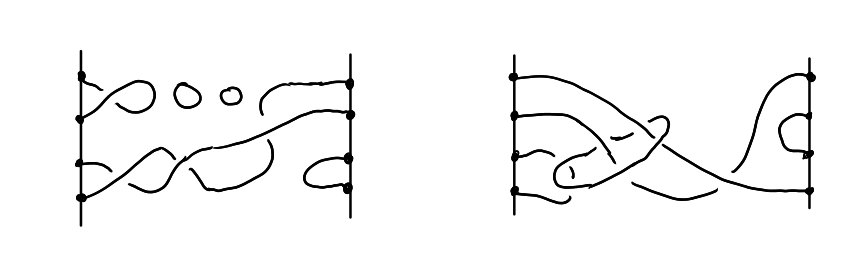
\includegraphics[scale=.25]{images/8.png}
\end{center}

\begin{remark}
\label{sec:temp-lieb-algebra}
  Any tangle diagram defined in this way (that is, the endpoints of strings on sides) can be turned into the general tangle diagram where the endpoints are on a circle. To see this, we simply connect the sides and expand it into a circle.
\end{remark}

Let $\Uplambda = \Z[A, A^{-1}]$ be the ring of Laurent polynomials and $\text{TA}_n(\delta)$ be a $\Uplambda$-algebra generated by $e_i$ for $1 \leq i \leq n$ satisfying the following relations 
\begin{align}
\label{eq:3}
\begin{split} 
  e_i^2 &= \delta e_i \\
  e_ie_{i\pm 1}e_i &= e_i \\
  e_ie_j &= e_je_i \hspace*{2em} \text{for } |i-j| > 1.
\end{split}
\end{align}
The $\Uplambda$-alegbra $\text{TL}_n(\delta)$ is called a Temperley-Leib algebra.

\begin{definition}
\label{sec:temp-lieb-algebra-1}
Let $R$ be a commutative ring and $\{ \gamma_n : B_n \to R \}_{n\geq 2}$ a sequence of functions such that the following conditions are satisfied.
\begin{enumerate}
\item\label{item:1} For two equivalent braids $\alpha, \beta \in B_n$ (equivalence under braid relations and isotopy), $\gamma_n(\alpha) = \gamma_n(\beta)$; 
\item\label{item:2} If $\alpha, \beta \in B_n$, then $\gamma_n(\beta) = \gamma_n(\alpha\beta\alpha^{-1})$ or equivalently, $\gamma_n(\alpha\beta) = \gamma_n(\beta\alpha)$;
\item\label{item:3} If $\beta \in B_n$, then there is a constant $a\in R$, independent of $n$, such that 
\begin{align}
\label{eq:5}
  \begin{split}
    \gamma_{n+1}(b\sigma_n) &= a \gamma_n(b) \\
    \gamma_{n+1}(b\sigma_n^{-1}) &= a^{-1} \gamma_n(b).
  \end{split}
\end{align}
\end{enumerate}
Then the sequence $\{\gamma_n\}$ is called a Markov trace on $\{B_n\}$.
\end{definition}

Let $\beta = \sigma_{i_1}^{r_{i_1}}\cdots\sigma_{i_k}^{r_{i_k}}$ be a braid in $B_n$. The writhe of $\beta$, denoted by $w(\beta)$, is defined to be the sum of the exponents $r_{i_1}, \ldots, r_{i_k}$. The Markov trace $\gamma_n\}$ can be used to construct invariants for links. Indeed, compare this with the Markov function we defined above.

\begin{theorem}
\label{sec:temp-lieb-algebra-2}
Let $\{ \gamma_n  \}$ be a Markov trace on $B_n$. Let $L$ be a link isotopic to a closed braid $\overline{\beta}$ (Alexander's theorem assures this). Set $\hat{\gamma}(L) = a^{-w(\beta)} \gamma_n(\beta) $. Then $\hat{\gamma}$ is an invariant for links.
\end{theorem}

The proof is quite similar to the one we wrote in the case of Markov functions. Observe that $w(\beta)$ is invariant under conjugation and braid isotopy and is used to cancel the effect of the second Markov move: $\beta \to \beta\sigma_n^{\pm 1}$.

Define $\left< \cdot \right> : B_n \to \Z[A, A^{-1}]$ such that the evaluation of $\left< \beta \right>$ is done on $\overline{\beta}$, the closed braid. By Alexander's theorem, we may reduce any given link $L$ to an isotopic closed braid $\overline{\beta}$. Given a closed braid $\overline{\beta}$, we may resolve all the crossings using the following skein relation.

\begin{align}
\label{eq:6}
\begin{split}
  \left<\KPB\right> &= A \left<\KPC\right> + A^{-1} \left<\KPD\right> \\
  \overline{\alpha} \coprod \KPA &= (-A^2 - A^{-2}) \overline{\beta}
\end{split}
\end{align}

A tangle is said be to reduced if there are no crossings and no additional loops. Indeed, using the skein relation given above any tangle can be reduced (if it is not already). Let $U_i$ for $1 \leq i \leq n-1$ be the tangles described below. See that they are tangles (just rotated by a right angle).
\vspace*{-.25em}
\begin{figure}[h]
  \centering
  \includegraphics[scale=.3]{images/tanglegenerators.png}
\end{figure}
\vspace*{-.25em}
Indeed, these $U_i$ are the generators all of reduced tangles, for one may write any reduced tangle as a composition of these $U_i$. Note that we are drawing the tangles in a special way (in a way very similar to geometric braid diagrams). The following relations are the abstraction of the isotopy of tangles.
\vspace*{-.25em}
\begin{figure}[h]
  \centering
  \includegraphics[scale=.3]{images/tanglerelations.png}
\end{figure}
\vspace*{-.25em}

The bracket $\left< \cdot \right>$ is defined for braids and tangles (later, we will see the same bracket extended to links). See that $\left< \sigma_i \right> = A\left< 1_n \right> + A^{-1}\left< U_i\right>$ where $1_n$ is the tangle with $n$ parallel strands. Similarly $\left< \sigma_i^{-1} \right> = A^{-1}\left< 1_n \right> + A\left< U_i \right>$ from the skein relation. We may omit $1_n$ and write $A\left< 1_n \right> + A^{-1}\left< U_i\right>$ as $A + A^{-1}\left< U_i\right>$.

  Let $A_n$ be an algebra over the ring $\mathbb{Z}[A, A^{-1}]$ of Laurent polynomials generated by the generators $U_i$ for $i = 1,\ldots, n-1$ and the following relations hold: 
\begin{align*}
  U_i^2 &= (-A^2-A^{-2}) U_i, \\
  U_iU_{i\pm 1}U_i &= U_i, \\
  U_iU_j &= U_jU_i, \hspace*{.6em} \text{if } |i-j|>1.
\end{align*}

See that $A_n$ is then the Temperley-Leib algebra $\text{TA}_{n-1}(-A^2-A^{-2})$. Suppose $U$ is a reduced tangle. If we take the closure of $U$, we get an unlink of trivial crossing-less components. Let $\sharp U$ be the number of components in this unlink minus $1$.

\begin{proposition}
\label{sec:temp-lieb-algebra-3}
The set $\{A + A^{-1}\left< U_i\right>\}$ for all $1 \leq i \leq n-1$ satisfy the braid relations.
\end{proposition}

Define a morphism $\rho_n : B_n \to A_n$ by 
\begin{align*}
  \sigma_i &\rightsquigarrow A + A^{-1}U_i, \\
  \sigma^{-1}_i &\rightsquigarrow A^{-1} + AU_i.
\end{align*}

The above proposition is equivalent to the following one.

\begin{proposition}
The map $\rho_n: B_n \to A_n$ is a representation of the braid group $B_n$.
\end{proposition}
\begin{proof}
It is easily checked that $\rho_n$ preserves the braid relations. That is, 
\begin{align*}
  \rho_n(\sigma_i)\rho_n(\sigma^{-1}_n) &= 1, \\
  \rho_n(\sigma_i\sigma_{i+1}\sigma_i) &= \rho_n(\sigma_{i+1}\sigma_i\sigma_{i+1}), \\
  \rho_n(\sigma_i\sigma_j) &= \rho_n(\sigma_j\sigma_i) \text{ if } |i-j|>1.
\end{align*}
Indeed, 
\begin{align*}
  \rho_n(\sigma_i)\rho_n(\sigma_i^{-1}) &= (A+A^{-1}U_i)(A^{-1} + AU_i) \\
                                        &= 1 + (A^{-2} + A^2)U_i + U_i^2 \\
                                        &= 1 + (A^{-2} + A^2)U_i + \delta U_i \\
                                        &= 1 + (A^{-2} + A^2)U_i + (-A^{-2} - A^2)U_i \\
  &= 1,
\end{align*}
\begin{align*}
  \rho_n(\sigma_i\sigma_{i+1}\sigma_i) &= (A+A^{-1}U_i)(A + A^{-1}U_{i+1})(A + A^{-1}U_i) \\
                                       &= (A^2 + U_{i+1} + U_i + A^{-2}U_iU_{i+1})(A + A^{-1}U_i) \\
                                       &= A^3 + AU_{i+1} + AU_i + A^{-1}U_iU_{i+1} + A^{-1}U_i^2 + AU_i + A^{-1}U_{i+1}U_i + A^{-3}U_iU_{i+1}U_i \\
                                       &= A^3 + AU_{i+1} + (A^{-1}\delta + 2A)U_i + A^{-1}(U_iU_{i+1} + U_{i+1}U_i) + A^{-3}U_i \\
                                       &= A^3 + AU_{i+1} + (A^{-1}(-A^2 - A^{-2}) + 2A + A^{-3})U_i + A^{-1}(U_iU_{i+1} + U_{i+1}U_i) \\
  &= A^3 + A(U_{i+1} + U_i) + A^{-1}(U_iU_{i+1} + U_{i+1}U_i),
\end{align*}
and as we can see, the final equation is symmetric in $i$ and $i+1$, and finally 
\begin{align*}
  \rho_n(\sigma_i\sigma_j) &= \rho_n(\sigma_i)\rho_n(\sigma_{j}) \\
                           &= (A+A^{-1}U_i)(A + A^{-1}U_j) \\
                           &= (A + A^{-1}U_j)(A + A^{-1}U_i) \\
  &= \rho_n(\sigma_j\sigma_i).
\end{align*}
This completes our proof that $\rho_n$ is a representation of the braid group.
\end{proof}

\begin{remark}
\label{sec:temp-lieb-algebra-4}
In the discussion above, the Temperley-Leib algebra $A_n$ was regarded as a $\Uplambda$-module. When we built the homomorphism $\rho_n: B_n \to A_n$, we regarded $A_n$ as a group under multiplication.
\end{remark}


The bracket polynomial (first introduced by Kauffman) is defined for knots and links using the same skein relation. Although it is not a link invariant (it fails to be invariant under the $\mathcal{R}^1$), we can normalize it so that it yields the famous Jones polynomial.

We shall now derive the bracket polynomial from our representation $\rho_n$ of the braid group. Let $\beta = \sigma^{a_1}_{i_1}\cdots \sigma^{a_k}_{i_k} \in B_n$ be some braid. Then
\begin{equation}
\rho_n(\beta) = \prod^k_{t=1} (A+A^{-1}U_{i_t})^{a_t} = \sum_s \langle \beta | s \rangle U_s,
\end{equation}
where $\langle \beta | s \rangle \in \mathbb{Z}[A, A^{-1}]$ is the coefficient of $U_s$ in the expansion of $\rho_n(\beta)$.

Define $\langle U_s \rangle = \delta^{\sharp U_s}$ and the bracket for the closed braid $\bar{\beta}$ by 
\begin{equation}
\langle \bar{\beta} \rangle = \sum_s \langle \beta | t \rangle \delta^{\sharp U_s}.
\end{equation}
Thus We have constructed a polynomial function for closed braids. This is the Kauffman bracket polynomial. As we can check, it fails to be invariant under Markov moves.

The bracket of the braid may be normalized as
\begin{equation}
  \langle \bar{\beta} \rangle = (-A^3)^{-w(\beta)} \sum_s \langle \beta | t \rangle \delta^{\sharp U_s}.
\end{equation}
  Given an oriented link $L$ in $\mathbb{R}^3$ we define 
\begin{equation}
V(L) = \langle \bar{\beta} \rangle,
\end{equation}
where $\beta$ is a braid whose closure is isotopic to $L$.

\begin{theorem}
The polynomial $V$ is a link invariant.
\end{theorem}
  
\begin{proof}
  Let $L$ and $L^{\prime}$ be two ambient isotopic links in $\R^3$. By Alexander's theorem, we can find two braids, $\beta$ and $\beta^{\prime}$ such that $L$ (resp. $L^{\prime}$) is isotopic to the closure of $\beta$ (resp. $\beta^{\prime}$). By Markov's theorem, $\bar{\beta}$ and $\overline{\beta^{\prime}}$ are related by a sequence of Markov moves. Therefore, it suffices to show that the normalized bracket $\langle \bar{\beta} \rangle$ is invariant under Markov moves. 
\begin{enumerate}
\item\label{item:8} For conjugation, we must check that $\langle \bar{\beta} \rangle = \left< \overline{\alpha\beta\alpha^{-1}} \right>$ for some $\alpha \in B_n$. It suffices to check that $\rho_n(\beta) = \rho_n(\alpha\beta\alpha^{-1})$. Since $\rho$ is a homomorphism, it suffices to check that $\rho_n(\beta) = \rho_n(\sigma_i\beta\sigma^{-1}_i)$. This can be checked by expansion: 
\begin{align*}
  \rho_n (\sigma_i\beta\sigma_i^{-1}) &= (A+A^{-1}U_i)\rho_n(\beta)(A^{-1} + AU_i) \\
                                      &= (A\rho_n(\beta) + A^{-1}U_i\rho_n(\beta) )(A^{-1} + AU_i) \\
                                      &= \rho_n(\beta) + (A^{-2} + A^2)U_i\rho_n(\beta) + U_i^2\rho_n(\beta) \\
                                      &= \rho_n(\beta) + (A^{-2} + A^2)U_i\rho_n(\beta) + (-A^{-2} - A^2)U_i\rho_n(\beta) \\
  &= \rho_n(\beta).
\end{align*}
\item\label{item:9} To show that the normalized bracket is invariant under $\beta \to \beta \sigma_n$, we first observe that $w(\beta \sigma_n) = w(\beta) + 1$. Then 
\begin{align*}
  \langle \overline{\beta\sigma_n}\rangle &= (-A^3)^{w(\beta) + 1} (\sum_t^{} \langle \beta | t \rangle \delta^{||U||})(A + A^{-1}\langle U_i \rangle) \\
                                          &= \langle \bar{\beta} \rangle (-A^3(A + A^{-1}\langle U_n \rangle)) \\
                                          &= \langle \bar{\beta} \rangle (-A^4 - A^2\langle U_n \rangle) \\
                                          &= \langle \bar{\beta} \rangle (-A^4 - A^2(-A^2 - A^{-2})) \\
                                          &= \langle \bar{\beta} \rangle (-A^4 + 1 + A^4) \\
  &= \langle \overline{\beta}\rangle.
\end{align*}
\item\label{item:7} Since $\rho_n$ is a braid representation, the possibility of equivalence in the braid group is also checked.
\end{enumerate}
This completes our proof that $V$ is an invariant for oriented links.
\end{proof}
